\chapter{Lec20 20220420}

Topics

\begin{enumerate}
    \item Jellium in RPA, Lindhard function
    \item Screening
    \item Plasmon
\end{enumerate}

Goals

\begin{enumerate}
    \item Computing the dielectric function in RPA
    \item Appreciating how screening and plasmons in metals arise in our formalism
\end{enumerate}

\section{RPA: recap}

Let us recap what we last considered before the one-week break. We consider the electrons in 3D continuum space interacting with the ``neutralized'' Coulomb
\[ \hat{V}=\frac{1}{2}\int{\frac{d^3pd^3p'd^3q}{\left( 2\pi \right) ^9}V\left( q \right) :\hat{\psi}_{p+q,\sigma}^{\dagger}\hat{\psi}_{p'-q,\sigma '}^{\dagger}\hat{\psi}_{p'\sigma '}\hat{\psi}_{q\sigma}:}\]
\[ V\left( q \right) =\begin{cases}
	\frac{4\pi e^2}{q^2},\quad \mathrm{if}\; q\ne 0\\
	0,\quad \mathrm{if}\; q=0\\
\end{cases}\]
where $V(q=0)=0$ follows from the cancellation from the uniform positive background, and corresponding the Hartree term
\begin{figure}[H]
    \centering
    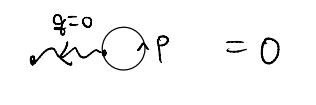
\includegraphics[width=\textwidth]{jupyterbook/data/fig/lec20-fig00.png}
\end{figure}
We motivated the RPA by asking how we might incorporate screening into our evaluation of the (finite-frequency) dielectric function. This could be understood by considering the Dyson's equation for the ``photon''
\begin{figure}[H]
    \centering
    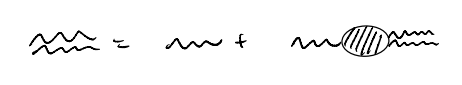
\includegraphics[width=\textwidth]{jupyterbook/data/fig/lec20-fig01.png}
\end{figure}
\[ V_{\mathrm{eff}}\left( q,\omega \right) =\frac{V\left( q \right)}{1+V\left( q \right) \chi \left( q,\omega \right)}\]
\begin{figure}[H]
    \centering
    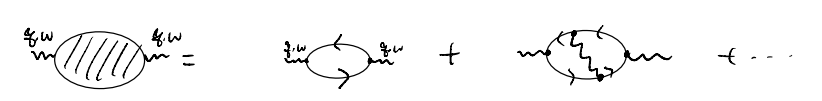
\includegraphics[width=\textwidth]{jupyterbook/data/fig/lec20-fig02.png}
\end{figure}
\[ i\chi \left( q,\omega \right) =i\chi _{\mathrm{RPA}}\left( q,\omega \right) +\cdots \]
Our main task for ``performing the RPA'' is, therefore, to evaluate
\begin{figure}[H]
    \centering
    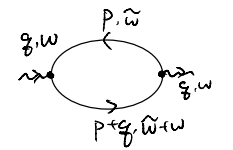
\includegraphics[width=0.3\textwidth]{jupyterbook/data/fig/lec20-fig03.png}
\end{figure}
\begin{align*}
    i\chi _{\mathrm{RPA}}\left( q,\omega \right) &=-\int{\frac{d\tilde{\omega}}{2\pi}\int{\frac{d^3p}{\left( 2\pi \right) ^3}\sum_{\sigma}{G_{\sigma}\left( p+q,\tilde{\omega}+\omega \right) G_{\sigma}\left( p,\tilde{\omega} \right)}}}\\
    &=-\left( 2S+1 \right) \int{\frac{d\tilde{\omega}d^3p}{\left( 2\pi \right) ^4}\frac{1}{\omega +\tilde{\omega}-\varepsilon _{p+q}+i\eta _{p+q}}\frac{1}{\tilde{\omega}-\varepsilon _p+i\eta _p}e^{i\tilde{\omega}0^+}}
\end{align*}
We could perform the frequency integral by noticing the function contains two poles, and closing the contour in the upper complex plane
\begin{figure}[H]
    \centering
    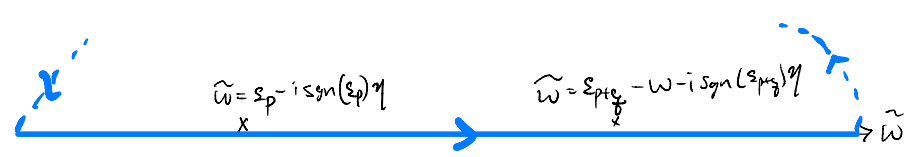
\includegraphics[width=\textwidth]{jupyterbook/data/fig/lec20-fig04.png}
\end{figure}
In particular, we enclose the poles only if they correspond to ``hole'' excitations (which live in the upper complex plane), i.e., the pole contribution in proportional to $n_k$:
\[ i\chi _{\mathrm{RPA}}\left( q,\omega \right) =-\left( 2S+1 \right) \frac{2\pi i}{2\pi}\int{\frac{d^3p}{\left( 2\pi \right) ^3}\left( \frac{n_{\vec{p}}}{\omega +\varepsilon _{\vec{p}}-\varepsilon _{\vec{p}+\vec{q}}}+\frac{n_{\vec{p}+\vec{q}}}{\varepsilon _{\vec{p}+\vec{q}}-\omega -\varepsilon _{\vec{p}}} \right)}\]
\[ \Rightarrow \chi _{\mathrm{RPA}}\left( q,\omega \right) =\left( 2S+1 \right) \int{\frac{d^3p}{\left( 2\pi \right) ^3}\frac{n_{\vec{p}}-n_{\vec{p}+\vec{q}}}{\varepsilon _{\vec{p}+\vec{q}}-\varepsilon _{\vec{p}}-\omega}}\]
Note that we have, with a sleight of hand, dropped the $i\eta$ factors. More later.

The integral above is called Lindhard function. Its evaluation is very similar to what we have seen for the Fock / exchange self-energy:
\begin{align*}
    \chi _{\mathrm{RPA}}\left( q,\omega \right) &=\left( 2S+1 \right) \int{\frac{d^3p}{\left( 2\pi \right) ^3}\left( \frac{n_{\vec{p}}}{\varepsilon _{\vec{p}+\vec{q}}-\varepsilon _{\vec{p}}-\omega}-\frac{n_{\vec{p}}}{\varepsilon _{\vec{p}}-\varepsilon _{\vec{p}-\vec{q}}-\omega} \right)}\\
    &=\frac{2S+1}{\left( 2\pi \right) ^3}\int_0^{k_F}{dp\int_0^{\pi}{d\theta p^2\sin \theta \int_0^{2\pi}{d\phi}}}\\
    &\quad \times \left( \frac{2m}{q^2+2pq\cos \theta -2m\omega}-\frac{2m}{2pq\cos \theta -q^2-2m\omega} \right)
\end{align*}
\[ \int_0^{\pi}{d\theta \sin \theta \frac{1}{a+b\cos \theta}}=\int_{-1}^1{du\frac{1}{a+bu}}=\frac{1}{b}\ln \left( \frac{a+bu}{a-bu} \right) \]
\begin{align*}
    \chi _{\mathrm{RPA}}\left( q,\omega \right) &=\frac{2S+1}{4\pi ^2}\int_0^{k_F}{dp\frac{p^2m}{pq}\left[ \ln \left( \frac{-2m\omega +q^2+2pq}{-2m\omega +q^2-2pq} \right) -\ln \left( \frac{-2m\omega -q^2+2pq}{-2m\omega -q^2-2pq} \right) \right]}\\
    &=\frac{\left( 2S+1 \right) mk_F}{4\pi ^2\tilde{q}}\int_0^1{d\tilde{p}\tilde{p}\left[ \ln \left( \frac{-\tilde{\omega}/\tilde{q}+\tilde{q}+2\tilde{p}}{-\tilde{\omega}/\tilde{q}+\tilde{q}-2\tilde{p}} \right) -\ln \left( \frac{-\tilde{\omega}/\tilde{q}-\tilde{q}+2\tilde{p}}{-\tilde{\omega}/\tilde{q}-\tilde{q}-2\tilde{p}} \right) \right]}
\end{align*}
\[ \tilde{p}=\frac{p}{k_F},\tilde{q}=\frac{q}{k_F},\tilde{\omega}=\frac{\omega}{k_{F}^{2}/2m}\]
\begin{align*}
    \int_0^1{dxx\ln \left( \frac{a+x}{a-x} \right)}&=\left. \frac{x^2}{2}\ln \left( \frac{a+x}{a-x} \right) \right|_{0}^{1}-\int_0^1{\frac{x^2}{2}\frac{2a}{a^2-x^2}dx}\\
    &=\frac{1}{2}\ln \left( \frac{a+1}{a-1} \right) +a\int_0^1{\left( 1-\frac{a^2}{a^2-x^2} \right) dx}\\
    &=\frac{1}{2}\ln \left( \frac{a+1}{a-1} \right) +a-\frac{a^2}{2}\int_0^1{\left( \frac{1}{a+x}+\frac{1}{a-x} \right) dx}\\
    &=\frac{1}{2}\ln \left( \frac{a+1}{a-1} \right) +a-\frac{a^2}{2}\left. \ln \left( \frac{a+x}{a-x} \right) \right|_{0}^{1}\\
    &=\frac{1}{2}\left( 1-a^2 \right) \ln \left( \frac{a+1}{a-1} \right) +a
\end{align*}
\[ \chi _{\mathrm{RPA}}\left( q,\omega \right) =\frac{\left( 2S+1 \right) mk_F}{4\pi ^2\tilde{q}}\left( a_++\frac{1}{2}\left( 1-a_{+}^{2} \right) \ln \left( \frac{a_++1}{a_+-1} \right) -\left( a_+\leftrightarrow a_- \right) \right) \]
\[ a_{\pm}=\pm \frac{\tilde{q}}{2}-\frac{\tilde{\omega}}{2\tilde{q}}\]
The prefactor could be simplified further using the 3D density of states (per spin)
\begin{align*}
    N_0&=\left. \frac{d}{d\varepsilon _k}\left( \frac{4\pi}{3}\frac{\left( 2m\varepsilon _k \right) ^{3/2}}{\left( 2\pi \right) ^3} \right) \right|_{k=k_F}\\
    &=2\pi \left( \frac{\sqrt{2m}}{2\pi} \right) ^3\sqrt{\varepsilon _{k_F}}\\
    &=\frac{2mk_F}{4\pi ^2};\quad \varepsilon _k=\frac{k^2}{2m}
\end{align*}
\begin{align*}
    \chi _{\mathrm{RPA}}\left( q,\omega \right) &=\frac{\left( 2S+1 \right) N_0}{2\tilde{q}}\left( \frac{1}{2}\left( 1-a_{+}^{2} \right) \ln \left( \frac{a_++1}{a_+-1} \right) -\left( a_+\leftrightarrow a_- \right) +\tilde{q} \right) \\
    &=\left( 2S+1 \right) N_0F\left( \tilde{q},\tilde{\omega} \right)
\end{align*}
\[ F\left( \tilde{q},\tilde{\omega} \right) =\frac{1}{4\tilde{q}}\left( 1-a_{+}^{2} \right) \ln \left( \frac{a_++1}{a_+-1} \right) -\left( a_+\leftrightarrow a_- \right) +\frac{1}{2}\]
The function $F(\tilde{q},\tilde{\omega})$ is known as the Lindhard function. Let us first consider its static limit
\[ \lim_{\omega \rightarrow 0} a_{\pm}=\lim_{\omega \rightarrow 0} \left( \pm \frac{\tilde{q}}{2}-\frac{\tilde{\omega}}{2\tilde{q}} \right) =\pm \frac{\tilde{q}}{2}\]
\begin{align*}
    F\left( \tilde{q},\tilde{\omega}=0 \right) &=\frac{1}{4\tilde{q}}\left( 1-\frac{\tilde{q}^2}{4} \right) \left[ \ln \left( \frac{\tilde{q}+2}{\tilde{q}-2} \right) -\ln \left( \frac{-\tilde{q}+2}{-\tilde{q}-2} \right) \right] +\frac{1}{2}\\
    &=\frac{1}{2\tilde{q}}\left( 1-\frac{\tilde{q}^2}{4} \right) \ln \left| \frac{\tilde{q}+2}{\tilde{q}-2} \right|+\frac{1}{2}
\end{align*}
Notice that, this time, we have a singularity at $\tilde{q}=2 \Rightarrow q=2k_F$ when the absolute value inside the log changes sign. We may plot it (the following by Wolfram alpha)
\begin{figure}[H]
    \centering
    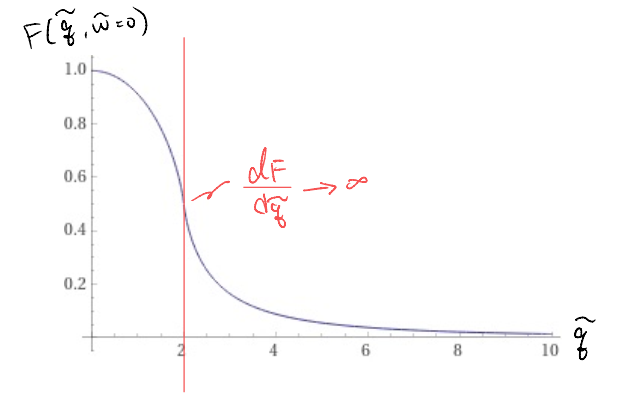
\includegraphics[width=\textwidth]{jupyterbook/data/fig/lec20-fig05.png}
\end{figure}
More generally, we obtain the RPA result for the dielectric function
\[ V_{\mathrm{eff}}\left( q,\omega \right) =\frac{V\left( q \right)}{1+V\left( q \right) \chi _{\mathrm{RPA}}\left( q,\omega \right)}=\frac{1}{\varepsilon _{\mathrm{RPA}}\left( q,\omega \right)}V\left( q \right) \]
\begin{align*}
    \Rightarrow \varepsilon _{\mathrm{RPA}}\left( q,\omega \right) &=1+V\left( q \right) \chi _{\mathrm{RPA}}\left( q,\omega \right) \\
    &=1+\frac{4\pi e^2}{q^2}\left( 2S+1 \right) N_0F\left( \frac{q}{k_F},\frac{\omega}{k_{F}^{2}/2m} \right)
\end{align*}

\section{Screening}

One interesting observation now is that, in the static limit,
\[ \lim_{q\rightarrow 0} \varepsilon _{\mathrm{RPA}}\left( q,\omega =0 \right) =\lim_{q\rightarrow 0} \left( 1+\frac{4\pi e^2}{q^2}\left( 2S+1 \right) N_0F\left( \frac{q}{k_F},\frac{\omega}{k_{F}^{2}/2m} \right) \right) \rightarrow +\infty \]
such divergence of the dielectric constant is characteristic of a metal, in which the charges always move to shield the interior from any possible external, static electric field. The picture may be clearer if we instead consider the effective interaction
\begin{align*}
    V_{\mathrm{eff}}\left( q,\omega =0 \right) &\stackrel{\text{RPA}}{=}\frac{V\left( q \right)}{1+V\left( q \right) \left( 2S+1 \right) N_0F\left( \frac{q}{k_F},0 \right)}\\
    &=\frac{4\pi e^2}{q^2+4\pi e^2\left( 2S+1 \right) N_0F\left( \frac{q}{k_F},0 \right)}\\
    &\stackrel{q\to 0}{\approxeq}\frac{4\pi e^2}{q^2+k^2}
\end{align*}
We may Fourier transform back to the real space, which gives (c.f. PS4)
\[ V_{\mathrm{eff}}^{\mathrm{static}}\stackrel{\text{RPA}}{=}\frac{e^2e^{-kr}}{r}\]
and we could interpret $k^{-1}=\frac{1}{\sqrt{4\pi e^2\left( 2S+1 \right) N_0}}$ as the length scale characterizing the screening of any stray charges in the metal. This is known as the Thomas-Fermi screening length.

\section{Plasmon}

As a second interesting observation, we consider the other order of the limits, in which we first send $q\to 0$ and keep $\omega$ finite. This order of limit might be considered by expanding the integrand directly
\begin{align*}
    \chi ^{\mathrm{RPA}}\left( q,\omega \right) &=\frac{\left( 2S+1 \right) N_0}{2\tilde{q}}\int_0^1{d\tilde{p}\tilde{p}\left[ \ln \left( \frac{-\tilde{\omega}/\tilde{q}+\tilde{q}+2\tilde{p}}{-\tilde{\omega}/\tilde{q}+\tilde{q}-2\tilde{p}} \right) -\ln \left( \frac{-\tilde{\omega}/\tilde{q}-\tilde{q}+2\tilde{p}}{-\tilde{\omega}/\tilde{q}-\tilde{q}-2\tilde{p}} \right) \right]}\\
    &=\frac{\left( 2S+1 \right) N_0}{2\tilde{q}}\int_0^1{d\tilde{p}\tilde{p}\ln \left( \frac{\left( \tilde{\omega}/\tilde{q} \right) ^2-\left( \tilde{q}+2\tilde{p} \right) ^2}{\left( \tilde{\omega}/\tilde{q} \right) ^2-\left( \tilde{q}-2\tilde{p} \right) ^2} \right)}\\
    &\Downarrow \omega \ne 0;q\rightarrow 0\\
    &=\frac{\left( 2S+1 \right) N_0}{2}\int_0^1{d\tilde{p}\tilde{p}\left( -\frac{8\tilde{p}\tilde{q}^2}{\tilde{\omega}^2}+O\left( \tilde{q}^4 \right) \right)}\\
    &\approx -\frac{4\left( 2S+1 \right) N_0}{3}\frac{\tilde{q}^2}{\tilde{\omega}^2}+O\left( \tilde{q}^4 \right) \\
    &=-\frac{4\left( 2S+1 \right) N_0}{3}\frac{q^2}{k_{F}^{2}\omega ^2}\frac{k_{F}^{4}}{4m^2}+O\left( \tilde{q}^4 \right) \\
    &=-\frac{\left( 2S+1 \right) k_{F}^{2}}{3m}\frac{mk_F}{2\pi ^2}\frac{q^2}{m\omega ^2}+O\left( \tilde{q}^4 \right) \\
    &=-n_0\frac{q^2}{m\omega ^2}+O\left( \tilde{q}^4 \right)
\end{align*}
\[ n_0=\frac{\left( 2S+1 \right)}{\left( 2\pi \right) ^3}\frac{4}{3}\pi k_{F}^{3}\]
where $n_0$ is the electron density. This gives the dielectric function
\[ \lim_{q\rightarrow 0} \varepsilon _{\mathrm{RPA}}\left( q,\omega \right) =1+\frac{4\pi e^2}{q^2}\left( -n_0\frac{q^2}{m\omega ^2}+O\left( \tilde{q}^4 \right) \right) =1-\frac{\omega _{p}^{2}}{\omega ^2}\left( 1+O\left( q^2 \right) \right) \]
where
\[ \omega _p=\sqrt{\frac{4\pi e^2n_0}{m}}\]
is the plasma frequency. This characterizes the time it takes for the electrons to respond to an oscillating electric field: while they screen stray charges completely in the static limit, such screening is ineffective when the field is changing at frequencies $\omega > \omega_p$ such that the electron distribution is not able to follow.

To get a more physical sense, let us try to put in some numbers. First we go from the CGS-ESU units to SI:
\[ \omega _p=\sqrt{\frac{4\pi e^2n_0}{m}}\rightarrow \sqrt{\frac{e^2n_0}{\varepsilon _0m}}\]
As an example, consider sodium
\[ \begin{cases}
	n_0=2.65\times 10^{22}cm^{-3}=2.65\times 10^{28}m^{-3}\\
	m=1.06m_e=9.656\times 10^{-31}kg\\
\end{cases}\]
and putting in
\[ \begin{cases}
	e^2/\varepsilon _0=0.29\times 10^{-26}kgm^3s^{-2}\\
	\hbar =6.58\times 10^{-16}eV\cdot s^{-1}\\
\end{cases}\]
We find
\[ \hbar \omega _p=5.87eV\]
In comparison, the visible spectrum is around $\sim 1.6-3.3 eV$. This explains why metals are shiny: visible light is not oscillating fast enough to penetrate, and it gets reflected.
